\documentclass{beamer}

\usepackage{graphicx}
\usepackage{hyperref}
\usepackage{listings}
\usepackage{tikz}

% beamer configuration
\mode<presentation> {
	\usetheme{Hannover}
}
\setbeamercolor{block title}{bg=yellow!50,fg=black}
\setbeamercolor{block body}{bg=yellow!10,fg=black}
\setbeamertemplate{enumerate subitem}[square]
\setbeamercovered{transparent}
\setbeamertemplate{frametitle}[default][left]
\AtBeginSection[]{
	\begin{frame}
		\vfill
		\centering
		\begin{beamercolorbox}[center]{title}
			\usebeamerfont{title}\insertsection\par%
		\end{beamercolorbox}
		\vfill
	\end{frame}
}

% listings configuration
\lstset{
	basicstyle=\footnotesize,
	showstringspaces=false
}

% tikz configuration
\tikzset{
	reg/.style = {
		shape=rectangle,
		draw,
		align=left,
		top color=blue!10,
		bottom color=blue!10
	}
}





\title[]{An Introduction to Web Development \\ with Flask}

\subtitle{\vspace{0.25in} 
\includegraphics[scale=0.15]{images/flask-logo.png}}

\author[]{Prudhvi Boyapalli}

\institute{
	Rice Computer Science Club \\
	Hack \& Learn Workshop \\
	January 13, 2017
}

\date{}

\begin{document}

\begin{frame}
	\titlepage
\end{frame}

\begin{frame}[t]{}
	\tableofcontents
\end{frame}

\section{Introduction}

\subsection{Flask}
	\begin{frame}[t]{How does a web app work? What does Flask do?}
		Flask is a Python microframework for building web applications.

		\begin{center}
		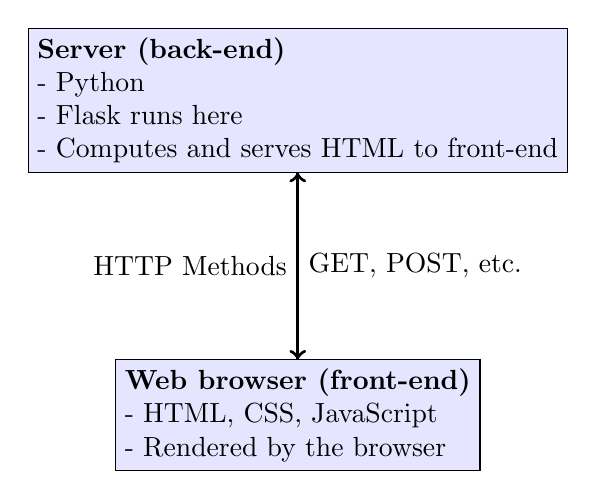
\begin{tikzpicture}
		\node[reg] (server) at (0,0) {
			\textbf{Server (back-end)}\\
			- Python\\
			- Flask runs here\\
			- Computes and serves HTML to front-end
		};
		\node[reg] (browser) at (0, -4) {
			\textbf{Web browser (front-end)}\\
			- HTML, CSS, JavaScript\\
			- Rendered by the browser
		};
		\draw[very thick, ->] (server) -- (browser)
			node [midway, left]{HTTP Methods};
		\draw[very thick, ->] (browser) -- (server)
			node [midway, right]{GET, POST, etc.};
		\end{tikzpicture}
		\end{center}
	\end{frame}


\subsection{Pre-reqs}
	\begin{frame}[t]{Necessary prior knowledge}
		\begin{itemize}
			\item{
				Basic familiarity with Python
				\begin{itemize}
					\item{If you've taken COMP140 you're in good shape}
				\end{itemize}
			}
			\pause
			\item{
				Basic familiarity with HTML and JavaScript, CSS
				\begin{itemize}
					\item{Be able to read HTML and JavaScript syntax}
					\item{CSS is optional}
				\end{itemize}
			}
		\end{itemize}
	\end{frame}


\subsection{Setup}
	\begin{frame}[t]{Install Python \& Flask}
		\begin{itemize}
			\item{
				Install Python if you haven't already: \url{python.org}
				\begin{itemize}
					\item{Either Python 2.7.9+ or 3.3+}
				\end{itemize}
			}
			\item{
				Install Flask using PIP
				\begin{itemize}
					\item{\textbf{P}ip \textbf{I}nstalls \textbf{P}ackages from
						the \textbf{Py}thon \textbf{P}ackage \textbf{I}ndex a.k.a. PyPI}
					\item{\texttt{pip} is included in the Python install}
				\end{itemize}
			}
		\end{itemize}
		\begin{block}{Flask Installation}
		\begin{semiverbatim}
			> sudo pip install Flask
		\end{semiverbatim}
		\end{block}
	\end{frame}


	\begin{frame}[t]{Editing}
		An IDE is overkill for this workshop. Use a programmer's editor that
		you're comfortable with:
		\begin{itemize}
			\item{Vim (All platforms)}
			\item{Atom (All platforms)}
			\item{Visual Studio Code (All platforms)}
			\item{Sublime Text (All platforms)}
			\item{Notepad++ (Windows)}
			\item{TextMate (OSX)}
			\item{Whatever floats your boat}
		\end{itemize}
	\end{frame}


	\begin{frame}[t]{Debugging}
		You'll be testing and debugging your code from the browser, so use one
		with good developer tools:
		\begin{itemize}
			\item{Chrome}
			\item{Firefox}
		\end{itemize}

		Other browsers can be used, but Chrome or Firefox will minimize the
		chance of running into browser specific issues.
	\end{frame}


\section[Hello World]{Hello World \newline (Open up your editor and follow along!)}

\subsection{Basic Example}
	\begin{frame}[t]{Super basic hello world example}
		This is the bare minimum code needed on the back-end to serve a web
		page
		\begin{block}{./code/hello\_world\_example/hello\_world.py}
			\lstinputlisting[language=Python]{../code/hello_world_example/hello_world.py}
		\end{block}
	\end{frame}


	\begin{frame}[t]{Running the web app}
		Once we've written the flask code, we can run the server locally and
		view the results in our web browser
		\pause

		\begin{block}{Execute these commands to run the code:}
			\begin{semiverbatim}
				> cd /directory/with/project

				> export FLASK\_APP=hello\_world.py

				> flask run
			\end{semiverbatim}
		\end{block}
		\pause

		\begin{block}{Then you'll see something like:}
			\begin{semiverbatim}
				* Serving Flask app "hello\_world"

				* Running on \url{http://127.0.0.1:5000/}

					(Press CTRL+C to quit)
			\end{semiverbatim}
		\end{block}
	\end{frame}

\subsection{Closer Look}
	\begin{frame}[t]{How did that work?}
		\setbeamercovered{}
		\begin{enumerate}
			\item{We started up a local flask server which is listening at
					IP address 127.0.0.1, port 5000}
			\pause
			\item{We visited this page and the browser sent a request to our
					flask server}
			\pause
			\item{Because we visited \url{127.0.0.1:5000/} (emphasis on the
					\texttt{"/"}), the method bound to \texttt{"/"} was invoked}
			\pause
			\item{The \texttt{hello()} method in \texttt{hello\_world.py} was
					executed and the return value is sent to the browser as
					HTML}
			\pause
			\item{The browser received the HTML and rendered the webpage}
		\end{enumerate}
	\end{frame}


\subsection{Variable Routing}
	\begin{frame}[t]{Interactive hello world with variable routing}
		Now that we have a basic idea of how flask works, we can do some cool
		stuff with routing:
		\begin{block}{./code/hello\_world\_example/hello\_user.py}
			\lstinputlisting[language=Python]{../code/hello_world_example/hello_user.py}
		\end{block}
	\end{frame}

	\begin{frame}[t]{Running the new and improved web app}
		\begin{block}{As before:}
			\begin{semiverbatim}
				> export FLASK\_APP=hello\_user.py

				> flask run

				* Serving Flask app "hello\_user"

				* Running on \url{http://127.0.0.1:5000/}

					(Press CTRL+C to quit)
			\end{semiverbatim}
		\end{block}
		\pause

		\begin{block}{Hello World}
			\url{http://127.0.0.1:5000/world}
		\end{block}

		\begin{block}{Hello $<$user$>$}
			\url{http://127.0.0.1:5000/user/Foo}

			\url{http://127.0.0.1:5000/user/Bar}
		\end{block}
	\end{frame}

\section[List Sort]{List Sort \newline (Don't try to code this up right now.)}
\subsection{Demo}
	\begin{frame}[t]{Quick Demo}
		\vfill
		\begin{center}
			\href{http://127.0.0.1:5000}{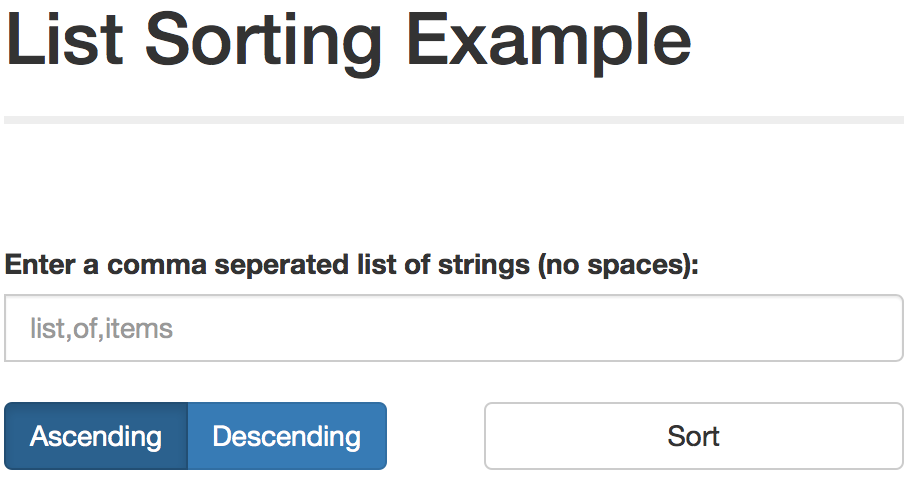
\includegraphics[scale=0.4]{images/list-sort.png}}
		\end{center}
		\vfill
	\end{frame}

\subsection{Structure}
	\begin{frame}[t]{Project Structure}
		As we build more complex web applications, we need to organize our
		files in a sensible way and maintain compatibility with flask \\

		\begin{block}{List Sort Project Structure}
			\footnotesize{\textit{Directories indicated in bold.}}
			\begin{itemize}
				\item{
					\textbf{list\_sort\_example}
					\begin{itemize}
						\item{
							\textbf{static}
							\begin{itemize}
								\item{
									\textbf{scripts} (JavaScript files)
								}
								\item{
									\textbf{styles} (CSS files)
								}
							\end{itemize}
						}
						\pause
						\item{
							\textbf{templates}
							\begin{itemize}
								\item{index.html}
							\end{itemize}
						}
						\pause
						\item{
							list\_sort.py
						}
					\end{itemize}
				}
			\end{itemize}
		\end{block}
	\end{frame}

\subsection{Communication}
	\begin{frame}[t]{\textbf{H}yper\textbf{t}ext \textbf{T}ransfer
			\textbf{P}rotocol}
		\textit{The data transfer protocol used on the World Wide Web}

		\begin{description}
			\item[GET]{
					The most common HTTP method, used to get files from a
					server. Multiple GET requests are made by your browser
					every time you visit a webpage to retrieve all the
					necessary resources needed to render that page, such as
					HTML files, CSS and JavaScript files, images, etc.
					\vspace{0.15cm}
				}
			\pause
			\item[POST]{
				This method is used to send data to a server. Commonly
				used to submit form data or any other user input.
			}
		\end{description}
		\pause

		\vspace{0.25cm}
		These are the most common HTTP request methods and the ones used by the
		demo, others exist: \\
		\vspace{0.15cm}
		\url{developer.mozilla.org/en-US/docs/Web/HTTP/Methods}
	\end{frame}

\subsection{Putting It All Together}
	\begin{frame}[t]{Putting It All Together (part 1)}
		\setbeamercovered{}
		\textit{Retrieving resources and rendering the webpage}
		\begin{enumerate}
			\item{User enters the address into their browser}
			\pause
			\item{Browser sends a \texttt{GET} request to the address, in this case
					\texttt{127.0.0.1:5000/}}
			\pause
			\item{The flask method bound to \texttt{"/"} is invoked and returns
					\texttt{index.html}}
			\pause
			\item{Browser processes the HTML file, which instructs it to load
					CSS and JavaScript files}
			\pause
			\item{Browser sends additional \texttt{GET} requests to the
					location indicated within the HTML files}
			\pause
			\item{Flask serves the static CSS and JavaScript files}
			\pause
			\item{Browser now has all necessary files and renders the webpage}
		\end{enumerate}
		\pause

		\large{\textbf{This all happens within milliseconds!}}
	\end{frame}

	\begin{frame}[t]{Putting It All Together (part 2)}
		\setbeamercovered{}
		\textit{Send data to the server, back-end computation, return results}
		\begin{enumerate}
			\item{User enters information into the input fields and clicks
					the \texttt{Sort} button}
			\pause
			\item{The JavaScript function bound to that button is invoked}
			\pause
			\item{The input information is read from the input
					fields and stored in an object
					(\textbf{J}ava\textbf{S}cript \textbf{O}bject
					\textbf{N}otation)}
			\pause
			\item{A \texttt{PUT} request is created and sent to
					\texttt{"/sort"}}
			\pause
			\item{Flask server receives the request
				\begin{enumerate}
					\item{The method bound to \texttt{"/sort"} is
							invoked}
					\pause
					\item{The data from the request object is
							accessed}
					\pause
					\item{The list is sorted}
					\pause
					\item{A response object is created with the results in JSON
							format and returned}
				\end{enumerate}
			}
			\pause
			\item{Back in the JavaScript function, the response is parsed}
			\pause
			\item{The necessary HTML to display the sorted list is created and inserted into page}
		\end{enumerate}
	\end{frame}

\section{Deep Dive}

\section{Conclusion}

\subsection{Summary}
	\begin{frame}[t]{Topics Covered}
		\begin{itemize}
			\item{Setting up a development environment for Flask}
			\item{Basic \& and variable routing}
			\item{\texttt{GET} and \texttt{POST} requests}
			\item{Accessing request data}
			\item{Overview of in-browser developer tools}
			\item{Building and serving a ``complex'' web app with HTML, CSS,
					JavaScript and Python}
		\end{itemize}
	\end{frame}


	\begin{frame}[t]{Next Steps}
		\begin{block}{More Flask Features}
			\begin{itemize}
				\item{URL Building}
				\item{Additional HTTP Methods}
				\item{HTML templates with placeholders, complex templating
						language}
				\item{File uploads}
				\item{Reading and writing cookies}
				\item{Redirects and error handling}
				\item{Managing sessions}
				\item{And lots of other stuff}
			\end{itemize}
		\end{block}

		 The Flask website and documentation is really good! Lots of great
		 tutorials exist, just search around.
	\end{frame}

	\begin{frame}[t]{Deploying your web app}
		Once you've developed and tested you app locally, you can deploy
		your code and make it publicly accessible. There lots of
		tutorials on how to do this for various cloud providers (AWS,
		Azure, DigitalOcean, etc).
	\end{frame}


\subsection{Resources}
	\begin{frame}[t]{Resources}
		\begin{itemize}
			\item{
				\textbf{This presentation \& and all of the code}\\
				\indent \url{github.com/hack-rice/flask-tutorial}
			}
			\item{
				\textbf{Flask website \& awesome documentation}\\
				\indent \url{flask.pocoo.org}
			}
		\end{itemize}
	\end{frame}

\subsection{Contact}
	\begin{frame}[t]{Contact}
		Prudhvi Boyapalli
		\begin{itemize}
			\item{prb2 AT rice.edu}
		\end{itemize}
		\pause

		HackRice
		\begin{itemize}
			\item{Fall 2017}
			\item{Annual hackathon right here on campus}
			\item{Great way to hone your skills and make something cool}
		\end{itemize}
		\pause

		RiceApps
		\begin{itemize}
			\item{Work on a team of students to build useful applications}
			\item{Great way to gain hands on development experience}
			\item{\url{http://riceapps.org}}
		\end{itemize}
		\pause

		Rice CS Facebook Group
		\begin{itemize}
			\item{\url{https://facebook.com/groups/365985373415471}}
		\end{itemize}

		CS Club Facebook Page
		\begin{itemize}
			\item{\url{https://facebook.com/ricecsclub}}
		\end{itemize}
	\end{frame}

\end{document}
